\documentclass[letter,11pt]{article}

\usepackage{fullpage}
\usepackage{hyperref}
\usepackage{graphicx}
\usepackage{multirow}
\usepackage{array}
\usepackage{adjustbox}

\newcommand{\niceurl}[1]{\href{#1}{\textsl{#1}}}
\newcommand{\code}[1]{\textsl{#1}}

\author{Dustin Lang}
\date{Aug 22, 2017}
\title{Evaluation of coadded and single-frame photometry methods}

\begin{document}
\maketitle

This report describes some simple experiments to evaluate the
signal-to-noise performance of coadding and single-frame photometry
methods.  The script for these experiments is publicly
available\footnote{%
  \niceurl{https://github.com/dstndstn/euclid/blob/master/coadd.py}}
and uses the \code{Tractor} code\footnote{%
  \niceurl{https://github.com/dstndstn/tractor}} to generate synthetic images.

The main question to be answered in this experiment is how much
signal-to-noise is lost (how much extra error is introduced) when
images are coadded before performing photometry, as compared to
performing photometry on single exposures.

This experiment assumes we are doing forced photometry on two
ground-based images.  That is, it assumes that we have a high-quality
catalog (eg, from Euclid VIS) in which we have detected a single point
source.  It assumes that we have correctly calibrated the astrometry
of the ground-based images, so we know exactly where in pixel
coordinates the point source will be found; and it also assumes that
we have a correct point-spread function (PSF) model for each image.
It assumes the two image were taken with the same bandpass filter, and
asks how well we can measure the flux of the point source in the
images.  We will vary the PSFs and the per-pixel noise.  In typical
ground-based images, the per-pixel noise is due primarily to the
Poisson distribution of the sky background, which is well approximated
by Gaussian noise; readout noise adds to this, but is usually fairly
small in comparison.  We will assume that the images have been
photometrically calibrated so that they are all in the same units;
thus longer exposures would result in the same measured flux values
but will have smaller per-pixel noise and smaller errors in the
measured fluxes.

We examine four cases, building up to the most realistic:
\begin{itemize}
\item \textbf{Case 1}: the two images have the same per-pixel noise,
  and the same PSF
\item \textbf{Case 2}: the two images have different levels of
  per-pixel noise, but the same PSF
\item \textbf{Case 3}: the two images have the same per-pixel noise
  but different PSFs
\item \textbf{Case 4}: the two images have different per-pixel noise
  and PSF (but the same per-image signal-to-noise).
\end{itemize}

For each of these four cases, we show results for three different
photometry methods.  In all cases, we are doing model-based forced
photometry: we are fitting for the flux where our pixel-space image
model best matches the observed pixels, given the per-pixel noise in
the images.
% This saturates the Cram\'er--Rao bound, meaning that it
% extracts all the available information in the images.
\begin{itemize}
  \item \textbf{Method A: Simultaneous fitting}: We do a single fit
    for the flux that produces the best match to both images at the
    same time.  That is, we are finding the flux that produces the
    smallest sum of chi-squared differences between the model and the
    images, summing the chi-squared of both images.
  \item \textbf{Method B: Single-frame average}: We fit for the flux
    in each image independently, and then compute a weighted average
    of the fluxes.  That is, we compute a best-fit flux for each
    image, and then average the flux measurements in ``catalog
    space''.
  \item \textbf{Method C: Coadding}: We add together the pixels of the
    two images (with weights), and then fit for the flux that best
    matches the coadded image.  When doing the fit, we compute the
    correct PSF model for the coadded images.  We test different
    \emph{coadd weights} $\alpha$, where the coadd is $C = \alpha A +
    (1 - \alpha) B$ for images $A$ and $B$, and the sum is pixelwise.
\end{itemize}

\begin{figure}[h!]
  \begin{center}
    \begin{tabular}{*{3}{c}}
      Method A
      &
      Method B
      &
      Method C
      \\
      \adjustimage{width=0.2\textwidth,valign=T}{method-a}
      &
      \adjustimage{width=0.2\textwidth,valign=T}{method-b}
      &
      \adjustimage{width=0.2\textwidth,valign=T}{method-c}
      \\
    \end{tabular}
  \end{center}
  \caption{ Schematics of the three photometry methods presented in
    this report.  Method A is simultaneous fitting: the flux is
    optimized to minimize the sum of chi-squared values between the
    model and data, summed over both images.  Method B measures a flux
    for each image (by minimizing chi-squared in the single image),
    then averages the two flux measurements.  Method C computes a
    coadd (averages the images), then fits a flux to the coadd.
    \label{fig:methods}
  }
\end{figure}

Note that Method A, simultaneous fitting, saturates the Cram\'er--Rao
bound, meaning that it extracts all the available information in the
images.  It is the most expensive in terms of computation time and
memory; it requires that all the images to be measured are in memory
at once.  We include it in this experiment only for comparison; one of
the results of this report is that Method B always performs exactly
the same.  This is because the flux measurements are sufficient
statistics and are distributed as Gaussians, so they can be combined
at ``catalog level'' with simple equations and no loss of information.
Method B has the strong advantage that each exposure is photometered
independently, so it is computationally cheap and embarrassingly
parallel.

\section*{Case 1: Same noise, same PSF}

\begin{figure}[h!]
  \begin{center}
    %\begin{tabular}{cc}
    %\end{tabular}
    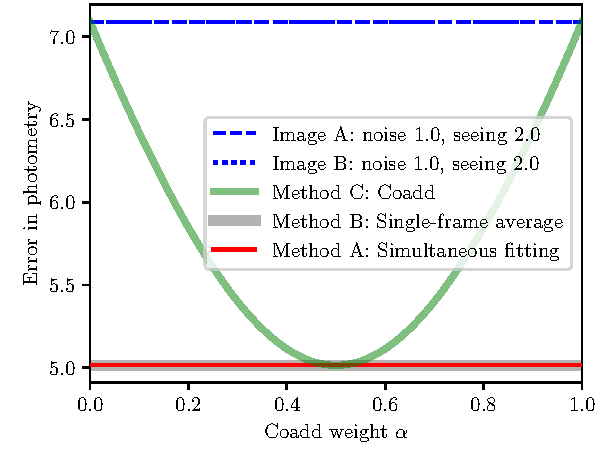
\includegraphics[width=0.48\textwidth]{coadd-00}
    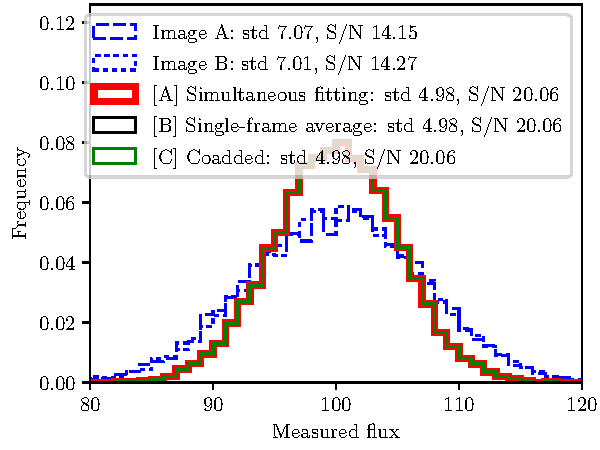
\includegraphics[width=0.48\textwidth]{coadd-01}
  \end{center}
  \caption{Results for Case 1 (same PSF, same per-pixel noise).  \textbf{Left}: the expected photometric
    uncertainty (error) for the different methods, as a function of
    the coadd weighting.  At the top of the plot, the two individual
    exposures, which have the same noise and PSF, have the same
    photometric error.  When the coadd weight is $\alpha = 0$ or $1$,
    the error in the coadd photometry equals that of the individual
    images.  With $\alpha = 0.5$, the coadd method performs as well as
    the other two methods.
    \newline \textbf{Right}: Results of simulations
    adding noise to synthetic images and running each of the
    photometry methods.  The measured fluxes are shown for $10,000$
    trials.  In this Case, the flux measurements on the individual
    exposures have a standard deviation of about 7, while all three
    of the other methods produce exactly the same results, with a standard
    deviation $1/\sqrt{2}$ as large; roughly 5.  Note that these results are
    entirely consistent with the analytically-computed expected performance values.
    \label{fig:caseone}}
\end{figure}


Figure~\ref{fig:caseone} shows results for Case 1.  In this case, all
three Methods produce exactly the same results.  Since the two images
have the same PSF and per-pixel noise, the best coadd weight $\alpha =
0.5$.


\section*{Case 2: Different noise, same PSF}

\begin{figure}[h!]
  \begin{center}
    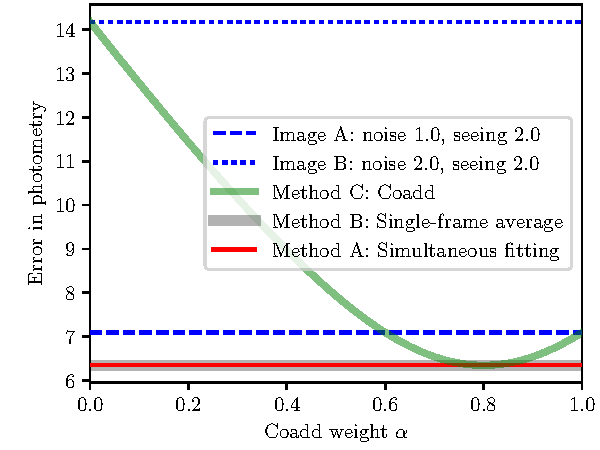
\includegraphics[width=0.48\textwidth]{coadd-02}
    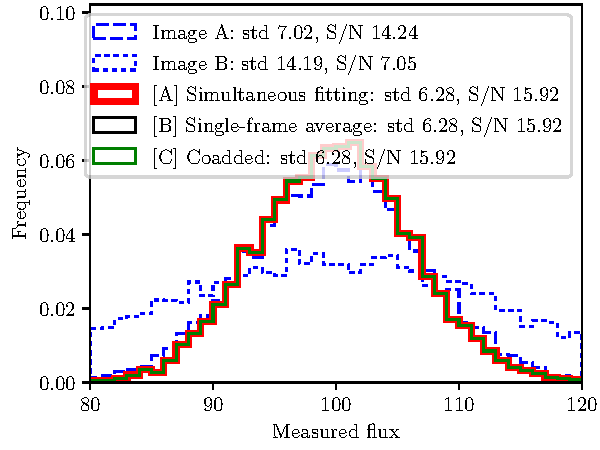
\includegraphics[width=0.48\textwidth]{coadd-03}
  \end{center}
  \caption{Results for Case 2 (same PSF, different per-pixel noise).
    \textbf{Left}: the expected photometric
    uncertainty (error) for the different methods, as a function of
    the coadd weighting.  Image A has half the per-pixel noise as Image B,
    so provides photometric measurements with half the uncertainty.
    The coadd weight that results in the best performance is $\alpha = 0.8$;
    this corresponds to inverse-variance weighting the images.
    \newline \textbf{Right}: Results of simulations where we
    add noise to synthetic images and run each of the
    photometry methods $10,000$ times.  The measured fluxes for
    the three methods are all identical, as in Case 1.
    \label{fig:casetwo}}
\end{figure}

In Case 2, one image has half the per-pixel noise as the other.
Results are shown in Figure~\ref{fig:casetwo}.  In this case, again,
each of the three Methods produce the same results.  The best coadd
weight $\alpha$ is found to correspond to inverse-variance weighting
of the images: Image A, with half the noise, is given a weight four
times greater than that of Image B.



\section*{Case 3: Same noise, different PSF}

\begin{figure}[h!]
  \begin{center}
    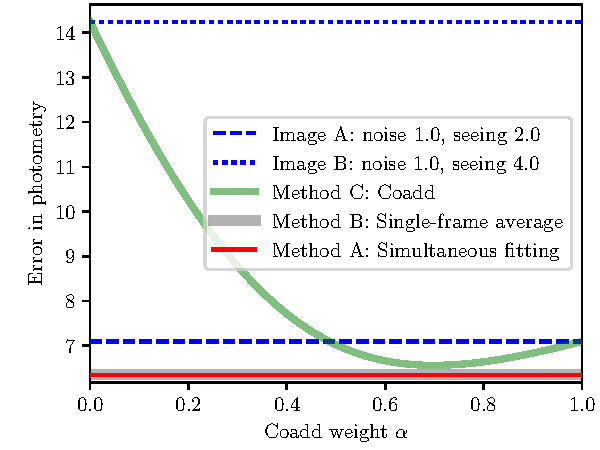
\includegraphics[width=0.48\textwidth]{coadd-04}
    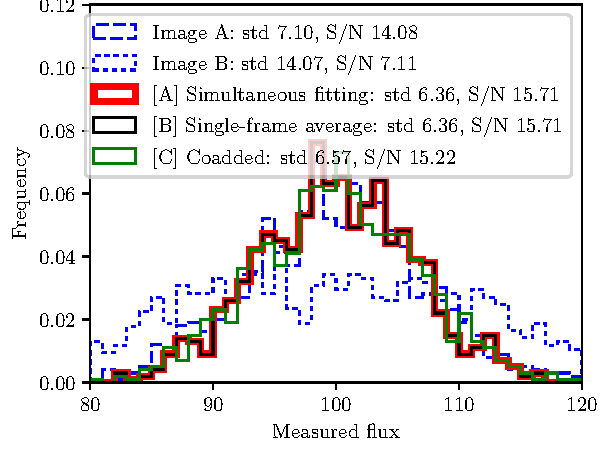
\includegraphics[width=0.48\textwidth]{coadd-05}
  \end{center}
  \caption{Results for Case 3 (same per-pixel noise, different PSF).
    \textbf{Left}: the expected photometric uncertainty (error) for
    the different methods, as a function of the coadd weighting.
    Image A has half the seeing size as Image B, and provides
    photometric measurements with half the uncertainty.  The coadd
    weight that results in the best performance is $\alpha \sim 0.7$.
    Even with the best coadd weight, the coadd method perform slightly
    worse than the other methods.  Since the majority of the
    signal-to-noise is carried by Image A, the difference is quite
    small.
    \newline \textbf{Right}: Results of simulations where we add noise
    to synthetic images and run each of the photometry methods
    $10,000$ times.  The measured fluxes for the three methods are as
    predicted: Methods A and B (simultaneous fitting or catalog-level
    averaging) still perform exactly the same, but Method C, coadding,
    performs slightly worse.
    \label{fig:casethree}}
\end{figure}

In Case 3, one image has half the seeing size (full-width at half-max)
as the other.  Results are shown in Figure~\ref{fig:casethree}.
Here, the coadding method performs slightly worse than the other methods.





\section*{xxx}


In this experiment, I am looking at four cases of doing forced photometry on two images:

Case 1: same noise, same PSF
Case 2: different noise, same PSF
Case 3: same noise, different PSF
Case 4: different noise, different PSF, but same per-image S/N

For each case, I have two plots:
- the first plot shows, as a function of the weighting used when adding the two images together (weight * image1 + (1-weight) * image2), what uncertainty you would get when doing force photometry on the coadd (smaller is better).

- the second plots shows histograms from running 10,000 rounds of drawing random noise, adding it to images, and running the different photometry methods.  Here, a tight distribution in flux values (narrower Gaussian) is better.

The photometry methods I'm showing are:
1. individual exposures, one at a time.
2. weighted-sum of the individual exposures (inverse-variance weighting)
3. simultaneous fitting of individual exposures.
4. create a coadd, and then photometer the coadd.

All the plots show that methods (2) and (3) perform exactly the same.  This is totally expected for Gaussian noise.

Looking at the four cases:

Case 1, where the noise and PSF are the same, shows that coadding with equal weights results in no loss of signal-to-noise, as you would expect.

Case 2 shows that when the noise levels differ but the PSF is the same, the best coadd weight is different than 50/50; it's 80/20 in this example -- it's an inverse-variance weighting.  With the optimal coadd weight, the performance of the coadd matches the performance of individual exposures.  This is also exactly as expected.

Case 3 shows that when the PSFs are different, the best coadd weight is some intermediate value, and, as we wanted to show, the best signal-to-noise you can deliver from a coadd is worse than you get from photometering the individual exposures.  In this case the loss of signal-to-noise is not very large because one of the images carries a lot more signal than the other, so no matter what you do the worse image doesn't add much.

Case 4 is really the punch line.  Here the PSFs are different, but the signal-to-noises in the two images are roughly equal.  This would happen in a survey with adaptive exposure times, where you expose for longer (or take more exposures) when the seeing is worse.  The two images contribute similar amounts of signal-to-noise, but their PSFs are quite different, so creating a coadd destroys information.

Even so, the amount of information lost is not that big -- S/N difference of about 5\%, or a 10\% difference in telescope time.  For CFIS and similar surveys that is a significant number of nights :)  But a factor of two in seeing values is probably extreme...


I would be very happy to get your comments on how to improve these experiments, plots, or explanation to best communicate this result to the group.

cheers,
--dustin



In your introduction you might want to frame this as simplified baby steps up to the reality case (case 4) which is the one that should dictate the final decision purely from a SNR consideration (then there is the filter response which is yet another, as strong, argument towards single frame photometry).

For:

1. individual exposures, one at a time.
2. weighted-sum of the individual exposures (inverse-variance weighting)
3. simultaneous fitting of individual exposures.
4. create a coadd, and then photometer the coadd.

-> in 2 you mean building the SNR out of the catalogs, a catalog coadd, (worth making this explicit since as written it evocates a bit some sort of image coadd).

-> Also for clarity of your text, rename that second batch of conditions a/b/c/d as you refer to 1/2/3/4 from above just below that paragraph.

For you plot, seeing 2.0 vs 1.0, I understand it is just a scaling factor (not 1" vs 2" in absolute?), this is worth mentioning, specially since sampling effect will likely start having an impact at some point (your study ignores a pixel grid I guess?).

Regarding the conclusion, a factor of 2 in IQ is what we get in CFIS-r actually, max limit is 0.9 but we have quite a few images <0.45". The SNR per exposure being however derived for a point source in a 2" diameter aperture, it is the sky background that influences most the SNR per exposure, here a factor of ~two is part of the plan (dark vs grey sky as defined for MegaCam, you are likely to have a greater range on DECam considering your airmass right?).

You have a wealth of stats from DECaLS on your dynamic integration in your three bands, if you want to add a practical illustration of your point? And you are absolutely right in pointing out 5 to 10% difference in observing time matters a lot. Considering how we scaled our ground surveys "how bad can they be while still enabling the photo-z?", any gain is good - Marc Sauvage is very receptive to this sort of statement.

Great punch line/conclusion for sure!

Jean-Charles.

\end{document}
